% ---------------------------- Preamble starts here ----------------------------

\documentclass[aspectratio=169]{beamer} %Remove [aspectratio=169] to get non-wide 4:3 slide aspect ratio

% --- Set beamer theme
\usetheme{Metropolis}
\setbeamertemplate{footline}{}				% Remove automatic footer
\setbeamertemplate{navigation symbols}{}	% Comment this line to display navigation symbols

% Load i2i symbol
\addtobeamertemplate{frametitle}{}{%
\begin{textblock*}{\linewidth}(0cm,7.4cm) % Replace with (0cm, 8cm) if using non-wide slide aspect
	
\includegraphics[width=\linewidth]{../../Common-Resources/img/Footer.png}
\end{textblock*}}

% --- Load packages
\usepackage{textpos}		% To align objects correctly
\usepackage{multicol}		% To right in multiple columns
\usepackage{color}			% To color text

% --- Add your information here
\title{An intro to Git and GitHub - Contributor Role}
\author{DIME Analytics}
\institute{DIME - The World Bank - \trainingURL{https://www.worldbank.org/en/research/dime}}
\date{\today}

\newcommand{\trainingURL}[1]{{\color{blue}\url{#1}}}

\newcommand{\traininerUsername}{kbjarkefur}
\newcommand{\repoName}{\traininerUsername/lyrics\_Nov14}
\newcommand{\trainingRepoURL}[1]{\trainingURL{github.com/\repoName #1}}
\newcommand{\trainerEmail}{\trainingURL{kbjarkefur@worldbank.org} }


% ---------------------------- Preamble ends here ----------------------------

\begin{document}

\begin{frame}

\includegraphics[width=\textwidth]{../../Common-Resources/img/Header.png}
\vspace{-0.2cm}
\titlepage 	 % Opening slide, prints inform
\end{frame}

\begin{frame}
\frametitle{Before the session starts:}
	\begin{enumerate}
		\item Do you have a GitHub.com account? If not, got to \trainingURL{https://github.com/join} and sign up
		\item Have you sent your GitHub username to the organizer or to \trainerEmail?
		\item Have you installed GitHub Desktop? If not got to \trainingURL{https://desktop.github.com/} and download it.
		\item Have you logged in at least once on GitHub Desktop? If not open GitHub Desktop and log in using your GitHub account.
		\item Have you been invited to \trainingRepoURL{} ? 
		\item And have you accepted at \trainingRepoURL{/invitations} ? 
	\end{enumerate}

\end{frame}

\begin{frame}

\includegraphics[width=\textwidth]{../../Common-Resources/img/Header.png}
\vspace{-0.2cm}
\titlepage 	 % Opening slide, prints inform
\end{frame}

\begin{frame}
	\frametitle{Three common GitHub roles}
	
	\small The objective of this training is to make you able to take the role of a Contributor. See DIME Analytics GitHub Roles for full details.
	
	

\begin{columns}[T] 
	\column{.33\textwidth} % Left column and width
	\Large \center{\textbf{Observer}}
	\begin{itemize}
		\small \item Browse code in GitHub
		\small \item Provide feedback through GitHub
		\small \item \textbf{Who?} Typically a PI that does not code
	\end{itemize}
	
	\column{.33\textwidth} % Middel column and width
	\Large \center{\textbf{Contributor}}
	\begin{itemize}
		\small \item Contribute to code in GitHub
		\small \item Understand and follow instructions from a Repo Maintainer
		\small \item \textbf{Who?} Typically an RA, or a PI that codes
	\end{itemize}
	
	\column{.33\textwidth} % Right column and width
	\Large \center{\textbf{Repo Maintainer}}
	\begin{itemize}
		\small \item Make sure that best practices and standards are followed in the repository
		\small \item Guide new contributors
		\small \item \textbf{Who?} Typically the most senior RA. Takes too much time for a PI.
	\end{itemize}
	
\end{columns}
	




\end{frame}

\begin{frame}
\frametitle{What is Git used for?}

	\begin{columns}[c] 
		
		\column{.60\textwidth} % Left column and width
		\begin{itemize}
			\item Git solves the \textit{Final.doc} problem
			\item <2->Common solution to the \textit{Final.doc} problem. Name all your docs like \textit{YYMMDD\_docname\_INITIALS.doc}
			\item <3->Git tracks \textit{YYMMDD} and \textit{INITIALS} for all edits  without the user having to remember it
			\item <4->That's far from everything, Git also solves:
			\begin{itemize}
				\item <4->Conflicting copy problem (DropBox etc.)
				\item <4->I can't re-produce my Baseline report problem
				\item <4->Who wrote this code 4 years ago and why?
				\item <4->And much much more...
			\end{itemize} 
		\end{itemize}	
		
		\column{.40\textwidth} % Right column and width
		\begin{figure}
			\centering
			
\includegraphics[width=1\linewidth]{../../Common-Resources/img/finaldoc_cartoon}
			\label{fig:finaldoccartoon}
		\end{figure}
		
	\end{columns}
\end{frame}


\begin{frame}
	\frametitle{What is Git, GitHub and GitHub Desktop?}
	\begin{figure}
		\centering
		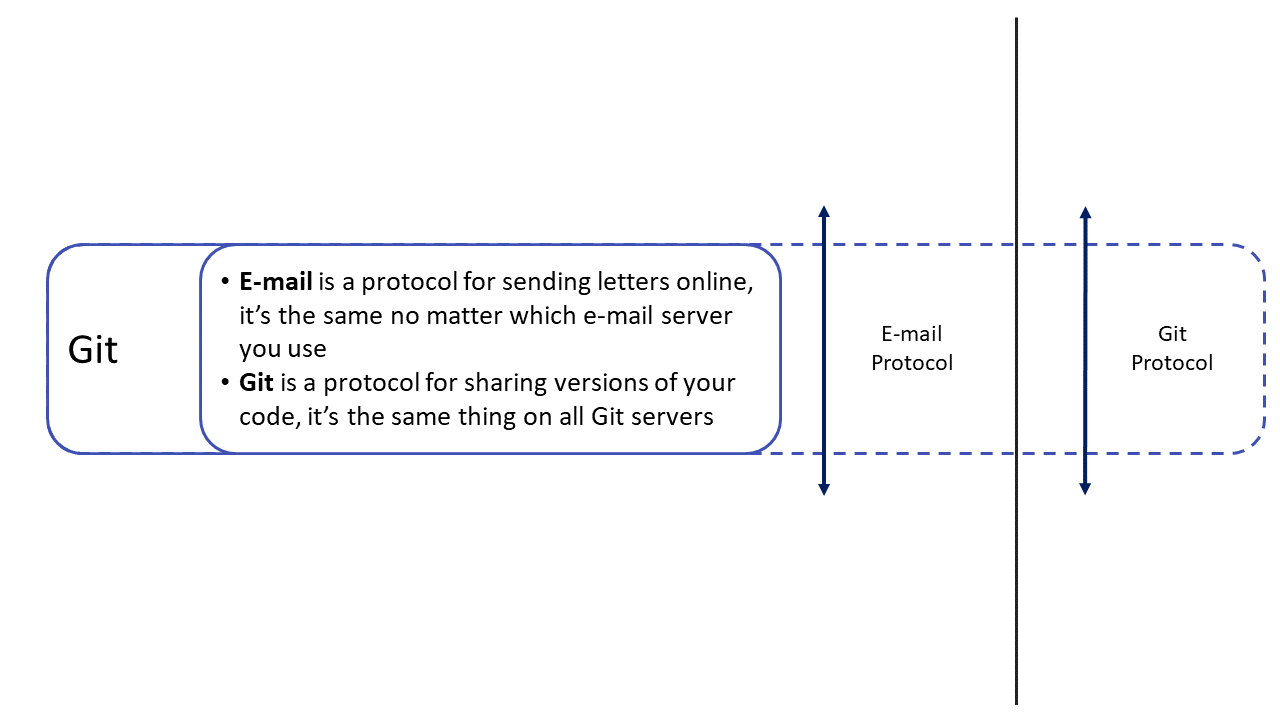
\includegraphics[width=0.7\linewidth]{../../Common-Resources/img/git_github_gitclient_git}
		\label{fig:gitgithubgitclient_git}
	\end{figure}
\end{frame}

\begin{frame}
	\frametitle{What is Git, GitHub and GitHub Desktop?}
	\begin{figure}
		\centering
		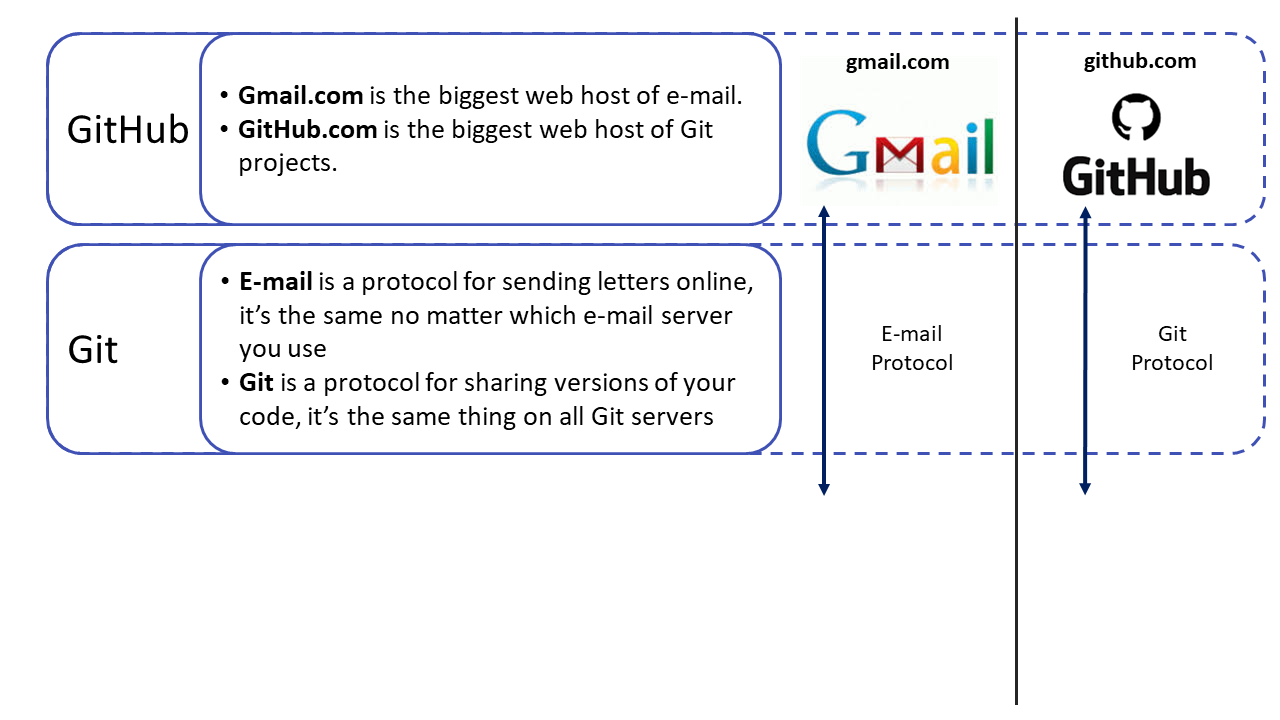
\includegraphics[width=0.7\linewidth]{../../Common-Resources/img/git_github_gitclient_github}
		\label{fig:gitgithubgitclient_github}
	\end{figure}
\end{frame}

\begin{frame}
	\frametitle{What is Git, GitHub and GitHub Desktop?}
	\begin{figure}
		\centering
		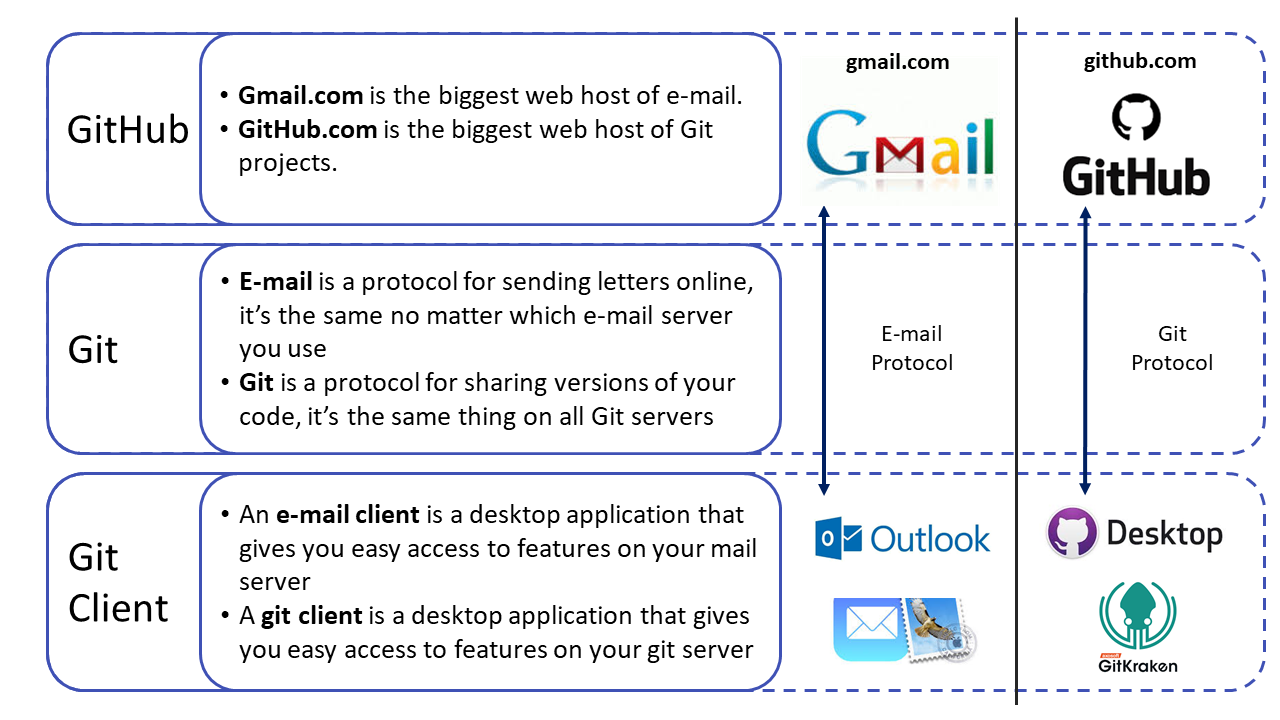
\includegraphics[width=0.7\linewidth]{../../Common-Resources/img/git_github_gitclient_gitclient}
		\label{fig:gitgithubgitclient_gitclient}
	\end{figure}
\end{frame}

\begin{frame}
\frametitle{What will we learn?}

	In the \textbf{An intro to Git and GitHub} you will learn to:
	
	\begin{itemize}
		\item Explore the history of a project folder in GitHub and see what different team members are currently working on
		\item Download a project folder from GitHub so you can work on it
		\item Create a space in the project folder where you can make your edits
		\item Make edits and share those versions with your team. When you are ready, request that your edits are included in the main version
	\end{itemize}

\end{frame}


\begin{frame}
\frametitle{MVO}

	\hspace*{2.5cm}\Large{Three Git concepts needed to do this:}
	
	\begin{itemize}
		\setlength{\itemindent}{3cm}
		\Large{\item Clone}
		\Large{\item Commit}
		\Large{\item Branch}
	\end{itemize}

\end{frame}


\begin{frame}
\frametitle{Code free training!}

	\begin{columns}[c] 
		
		\column{.15\textwidth} % Left column and width
		
		\column{.70\textwidth} % Left column and width
		\textbf{No code today!}
		
		\vspace{.5cm}
		
		We will not work with code today in our repository.
		
		\vspace{.25cm}
		
		Code tends to distract people if, for example, they see a command they do not understand. 
		
		\vspace{.25cm}
		
		Instead we will work with lyrics in .txt files that works exactly the same as code files in Git.
		
		\column{.15\textwidth} % Left column and width
		
	\end{columns}
\end{frame}

\begin{frame}
\frametitle{How to browse GitHub.Com}

	Your project folder is called a \textbf{repository} in Git. We will call the page you land on when you enter \trainingRepoURL{} the \textbf{main page}.
	
	\vspace{.5cm}

	\begin{columns}[T] 
	
		\column{.50\textwidth} % Left column and width
		GitHub.com -$>$ Repo
		\begin{enumerate}
			\item From anywhere on \trainingURL{github.com} click the \textit{octocat} icon in the top left corner.
			\item In the menu to your left you see the repositories you are invited to
			\item Click any repo to get to the main page of that repo.
		\end{enumerate}
		
		\column{.50\textwidth} % Left column and width
		Repo -$>$ Main page
		\begin{enumerate}
			\item Click the repo name in {\color{blue}\url{\repoName}} at the top of any page within the repo
			\item Click the tab that says \textbf{Code} below the repo name at any page in your repo
		\end{enumerate}
			
	\end{columns}
\end{frame}

\section{Clone}

\begin{frame}
\frametitle{What is cloning?}
	
	Cloning is similar to downloading a \textbf{repository} to your computer.
	
	\vspace{.5cm}
	
	The difference between cloning and downloading is that \textbf{when Git clones a repository it remembers where you downloaded it from}. This is necessary so that Git knows where to share the edits you make to the files in the repository.
	
\end{frame}

\begin{frame}
\frametitle{How do I clone a repository from GitHub?}
	
	\begin{columns}[c] 
		
		\column{.70\textwidth} % Left column and width
		How to clone a repository:
		\begin{enumerate}
			\item Go to the \textbf{main page} of \trainingRepoURL{}
			\item Click the green \textit{Clone or download} button (see image)
			\item Click \textit{Open in Desktop}
			\item Select where on your computer to clone the repository. Usually in your \textit{Documents} folder. Do \textbf{NOT} clone in a shared folder, like a network drive or in DropBox. 
		\end{enumerate}
		
		\column{.30\textwidth} % Left column and width
		\begin{figure}
			\centering
			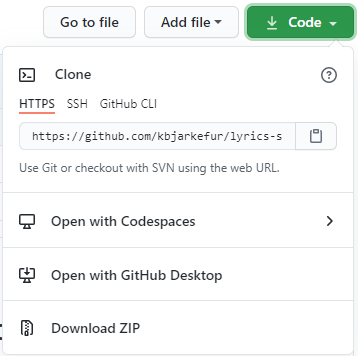
\includegraphics[width=1\linewidth]{img/clonedownload_button}
			\label{fig:clonedownloadbutton}
		\end{figure}
	
	\end{columns}

\end{frame}


\begin{frame}
\frametitle{Explore the clone}

	\begin{columns}[c] 
	
		\column{.20\textwidth} % Left column and width
		
		\column{.60\textwidth} % Left column and width
		\textbf{Explore the clone!}
	
		\vspace{.5cm}
	
		Compare the files and folders you cloned to your computer with those in the repository on \trainingRepoURL{}
		
		\column{.20\textwidth} % Left column and width
	
	\end{columns}

\end{frame}

\section{Collaboration on a Repository}

\begin{frame}
\frametitle{Explore the clone}

	\center{In order to collaborate on a repository we need to introduce two topics:}
	
	\vspace{1cm}
	
	\begin{columns}[c] 
		
		\column{.30\textwidth} % Left column and width
		\center{\huge{\textbf{Commits}}}
		
		\column{.30\textwidth} % Left column and width
		\center{\huge{\textbf{Branches}}}
		
	\end{columns}

	\vspace{2cm}

\end{frame}

\section{Commit}

\begin{frame}
\frametitle{What is a version in version control?}

	\begin{columns}[c] 
	
		\column{.50\textwidth}
		First look at how version control works in another software you might be familiar with
		
		\vspace{.5cm}
		
		In DropBox each saved version of a file is saved to the version history. This is the only way to do it automatically, but are all these versions meaningful differences?
		
		\column{.50\textwidth}
		\begin{figure}
			\centering
			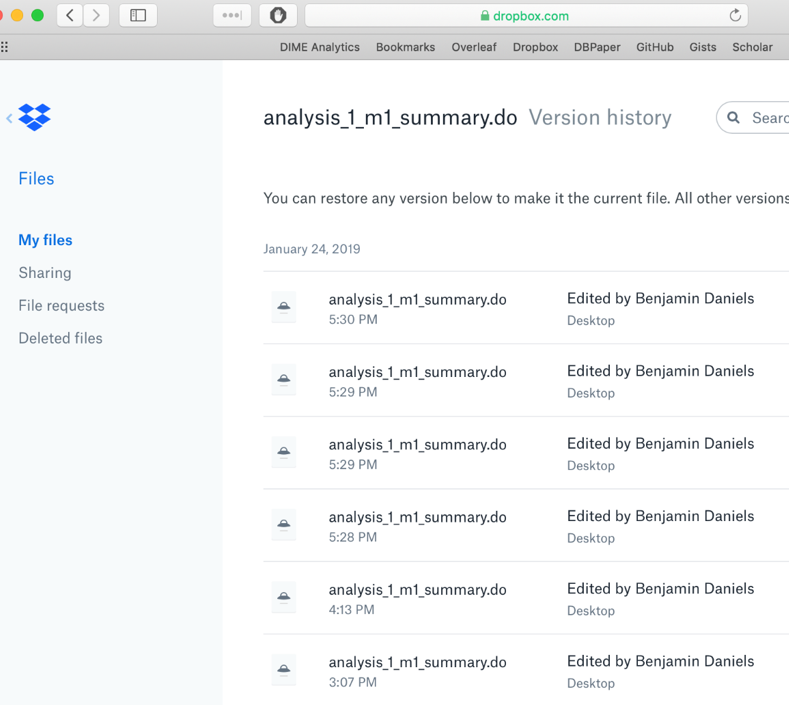
\includegraphics[width=1\linewidth]{../../Common-Resources/img/dropbox_versioncontrol}
			\label{fig:dropboxversioncontrol}
		\end{figure}
		
	\end{columns}


\end{frame}

\begin{frame}
\frametitle{What is a commit?}

	Instead of having a list of each saved version of a file, in Git we use \textbf{commits to indicate what is each meaningful difference between two versions of our project folder}. 
	
	\vspace{.25cm}
	
	Each commit is a snap shot of all files in the project folder, and lists how that snap shot differ from the previous snap shot (the previous commit).
	
	\vspace{.25cm}
	
	Each commit has a time stamp and tracks who did the commit. This is very similar to the \textit{YYMMDD\_docname\_INITIALS.doc} solution to the \textit{Final.doc} problem.

\end{frame}

\begin{frame}
\frametitle{How to make a commit}

	We need to introduce \textit{branches} before we can all commit to the same repository, so I for now, let me show you how to make a commit:
	
	\begin{enumerate}
		\item I add a new lyrics file in the clone
		\item I use GitHub desktop to commit the new file to the repository
		\item Can you see the new file on your computer?
		\item Can you see it if you sync in GitHub Desktop?
	\end{enumerate}	

\end{frame}


\begin{frame}
\frametitle{Exploring commits}

	Now when we know what a commit is, we can start exploring how the \trainingRepoURL{} repository was created.
	
	\vspace{.25cm}
	
	We will see a list of commits, that at first sight is similar to the the version history in DropBox, but \textbf{in Git the version list is more meaningful, as it is a list of only meaningful differences}.

	\vspace{.25cm}
	
	\begin{itemize}
		\item \trainingRepoURL{/commits}
		\item This list can also be found in GitHub Desktop
	\end{itemize}	

\end{frame}

\section{Branch}

\begin{frame}
\frametitle{Introducing branches}

	\begin{columns}[c] 
		
		\column{.60\textwidth}
		\textbf{Branches is the "killer feature" of Git}. This is where Git becomes really powerful as a collaboration tool and as version control.
		
		\vspace{.25cm}
	
		Branches allows you to \textbf{create a copy of the code where you can experiment}, if you like the result, \textbf{you can very easily merge your experiment with the main version of your code}.
		
		\vspace{.25cm}
		
		This non-linear version control is much more similar to how we actually work than the strictly linear version control in, for example, DropBox
		
		\column{.40\textwidth}
		\begin{figure}
			\centering
			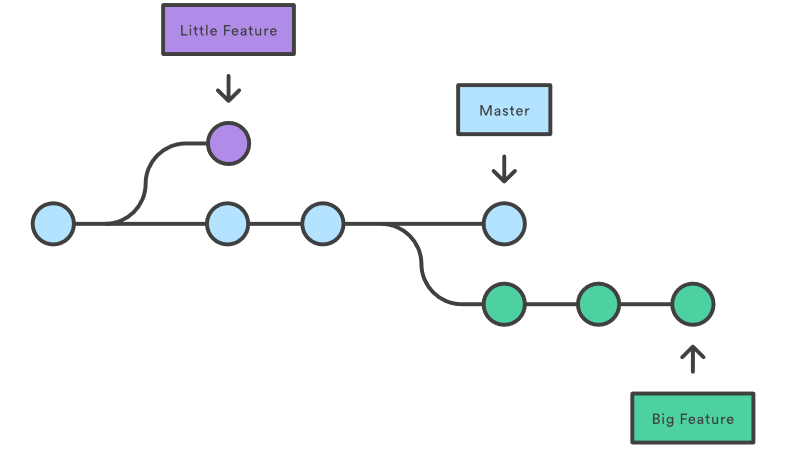
\includegraphics[width=1\linewidth]{../../Common-Resources/img/branches}
			\label{fig:branches}
		\end{figure}
		
	\end{columns}

\end{frame}

\begin{frame}
\frametitle{Looking at branches}


	\textbf{One more way to explore the repository}
	\begin{itemize}
		\item \trainingRepoURL{/commits} $<$- Linear progression
		\item \trainingRepoURL{/network} $<$- Non-linear progression
	\end{itemize}

	\vspace{.1cm}
	
	\textbf{Exploring branches}
	\begin{itemize}
		\item You can change branch in \textit{/commits}. What happens when you change branch?
		\item Go to the main page, what happens if you change branch here?
		\item Which version is in the clone on your computer? They are all actually in your clone, but only one is shown - \textbf{checked out} - at the time
		\item What happens to the content of the folder on your computer when you check out another branch in GitHub Desktop?
	\end{itemize}

\end{frame}

\begin{frame}
\frametitle{Working with branches}

	A typical Git work flow involves multiple branches and there are tools in GitHub to makes that work flow easy, but that is not within today's scope. Although, what you should know after this training is only how to create your own branch and how to commit to it. 
	
	\textbf{Create a branch:}
	\begin{itemize}
		\item Go to \trainingRepoURL{} and click the button where it says \textit{Branch: master}.
		\item Write your name in the field and click \textit{Create branch: your\_name}. Make sure it says \textit{from 'master'}.
		\item See how the button now says \textit{Branch: your\_name}
		\item Go to \trainingRepoURL{/network} to check that your branch is there.
	\end{itemize}	

\end{frame}

\section{Combining Commit \& Branch}

\begin{frame}
\frametitle{Now it is time to collaborate}

\textbf{Now it is time for you to collaborate:}
\begin{enumerate}
	\item Make sure your branch is checked out in GitHub Desktop.
	\item Open a text editor. It could be \textit{Notepad} if you are using Windows, \textit{TextEdit} if you are using Mac, or any other code editor like \textit{Atom}, or \textit{Notepad++} etc.
	\item Google the lyrics of your favorite song, and copy the lyrics to a new file in the text editor you just opened
	\item Save the lyrics in your local clone according to these instructions:
	\begin{itemize}
		\item Save the file in \textit{.txt} format (Especially Mac users, this is not always the default)
		\item Name the file after the title of the song
		\item Save it in the appropriate genre folder (create a new genre folder if needed)
	\end{itemize}
\end{enumerate}

\end{frame}

\begin{frame}
\frametitle{Do your first commit}

\begin{columns}[c] 

\column{.60\textwidth} % Left column and width

\begin{enumerate}
	\item Open the changes tab in GitHub Desktop
	\item GitHub Desktop tracks your clone and has noticed that you changed something in it
	\item Then you need to do the three steps required to commit a file to the repository:
	\begin{enumerate}
		\item Make sure the file you want to add is checked
		\item Write a commit message and click \text{Commit to master}
		\item Click the sync button
	\end{enumerate}
\end{enumerate}

\column{.40\textwidth} % Left column and width
\begin{figure}
	\centering
	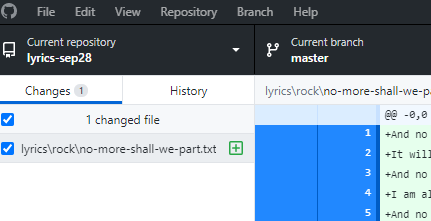
\includegraphics[width=1\linewidth]{img/desktop_changes}
	\label{fig:desktopchanges}
\end{figure}

\begin{figure}
	\centering
	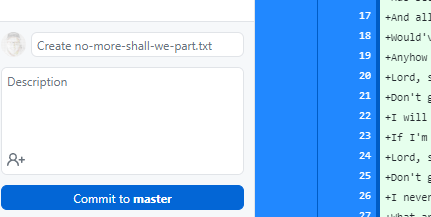
\includegraphics[width=1\linewidth]{img/desktop_commit}
	\label{fig:desktop_commit}
\end{figure}

\end{columns}

\end{frame}

\begin{frame}
\frametitle{Check your contribution}

	\textbf{Check your commit on GitHub:}
	\begin{itemize}
		\item Go to \trainingRepoURL{/network}
		\begin{itemize}
			\item Can you find your commit?
		\end{itemize}
		\item Go to \trainingRepoURL{/commits}
		\begin{itemize}
			\item Can you find your commit?
			\item If you cannot see your commit, make sure that you are looking in the correct branch
		\end{itemize}
	\end{itemize}

\end{frame}

\begin{frame}
\frametitle{Pull Requests}

	A feature related to branches is a \textbf{pull request}. When the edits you have done in your branch are ready to be merged with the main version of the code, you make a pull request, i.e. you are requesting that your edits are pulled into the master branch.
	
	
	A pull request can be made either by the person that edited the branch or the repo maintainer. 
	
	It is very common in GitHub repositories that only the repo maintainer have access to the master branch, and pull requests are then the only way to contribute to the master branch.  


\end{frame}

\begin{frame}
\frametitle{Merge your contribution}

	\textbf{To make a pull request for your branch:}
	\begin{itemize}
		\item Go to \trainingRepoURL{/pulls} and click \textit{New pull request}
		\item Make sure that the \textit{master} branch is selected as the \textit{base:} branch, and then select your branch as the \textit{compare:} branch
		\item Scroll down to check the edits you are requesting to be pulled in to the master branch. If it looks ok, then click \textit{Create pull request}
		\item Then you have the chance to add more instructions if you want, then click \textit{Create pull request} again 
	\end{itemize}
\end{frame}

\begin{frame}
\frametitle{Merge your contribution}

Can you see your lyrics file in the master branch now? Why not?

\vspace{.5cm}

Future trainings will teach you about merging pull requests. So I will do that for you now. Can you see your lyrics file in the master branch now?

\end{frame}



\begin{frame}
\frametitle{What have we learned?}
	
	In the \textbf{An intro to Git and GitHub} you have learned to:
	
	\begin{itemize}
		\item Explore the history of a project folder in GitHub and see what different team members are currently working on
		\item Download a project folder from GitHub so you can work on it
		\item Create a space in the project folder where you can make your edits
		\item Make edits and share those versions with your team. When you are ready, request that your edits are included in the main version
	\end{itemize}

\end{frame}

\begin{frame}
\frametitle{What have we learned?}

	In the \textbf{An intro to Git and GitHub} you have learned to:
	
	\begin{itemize}
		\item Explore the history of \textbf{repository} and see what different team members are currently working on
		\item \textbf{Clone} a \textbf{repository} so you can work on it
		\item Create a \textbf{branch} in the \textbf{repository} where you can make your edits
		\item Make edits and share \textbf{commits} with your team. When you are ready, make a \textbf{pull request} to the \textbf{master branch}
	\end{itemize}
\end{frame}

\section{Magic Trick}


\begin{frame}
\frametitle{Magic Trick}
	
	All great training ends with a magic trick! This is a pedagogical magic trick, don't worry, just bear with me!
	
	\vspace{1cm}
	
	\center{I need a volunteer for a simple task from the audience!}
	
	\vspace{1cm}

\end{frame}

\section{Next steps for the research team}

\begin{frame}
\frametitle{Three common GitHub Roles}
	
	

\begin{columns}[T] 
	\column{.33\textwidth} % Left column and width
	\Large \center{\textbf{Observer}}
	\begin{itemize}
		\small \item Browse code in GitHub
		\small \item Provide feedback through GitHub
		\small \item \textbf{Who?} Typically a PI that does not code
	\end{itemize}
	
	\column{.33\textwidth} % Middel column and width
	\Large \center{\textbf{Contributor}}
	\begin{itemize}
		\small \item Contribute to code in GitHub
		\small \item Understand and follow instructions from a Repo Maintainer
		\small \item \textbf{Who?} Typically an RA, or a PI that codes
	\end{itemize}
	
	\column{.33\textwidth} % Right column and width
	\Large \center{\textbf{Repo Maintainer}}
	\begin{itemize}
		\small \item Make sure that best practices and standards are followed in the repository
		\small \item Guide new contributors
		\small \item \textbf{Who?} Typically the most senior RA. Takes too much time for a PI.
	\end{itemize}
	
\end{columns}
	



	
\end{frame}

\begin{frame}
\frametitle{Next steps for the research team}

	Before adopting Git the research team should discuss the following things:

	\begin{itemize}
		\item Who will be repo maintainer
		\item Agree on a work flow
		\item Public/private repository
		\item External collaborators
		\item Where to put data and where to put code
		\item Request a World Bank repo to be set up
	\end{itemize}

\end{frame}

\begin{frame}{Useful links}
	\begin{itemize}
	  \item All DIME Analytics GitHub resources: \trainingURL{https://github.com/worldbank/dime-github-trainings}. For example:
		\begin{itemize}
			\item DIME Analytics GitHub Templates (for example .gitignore): \trainingURL{https://github.com/worldbank/dime-github-trainings/tree/master/GitHub-resources/DIME-GitHub-Templates}
			\item DIME Analytics GitHub Roles: \trainingURL{https://github.com/worldbank/dime-github-trainings/blob/master/GitHub-resources/DIME-GitHub-Roles/DIME-GitHub-roles.md}
		\end{itemize}
		\item Markdown cheat sheet (how to format text on GitHub.com):  \trainingURL{https://www.markdownguide.org/cheat-sheet/}
		\item DIME GitHub Account admin info and instructions: \trainingURL{https://github.com/dime-worldbank/dime-account-admin}
	\end{itemize}
\end{frame}



\end{document}
